\def\layersep{2.5cm}
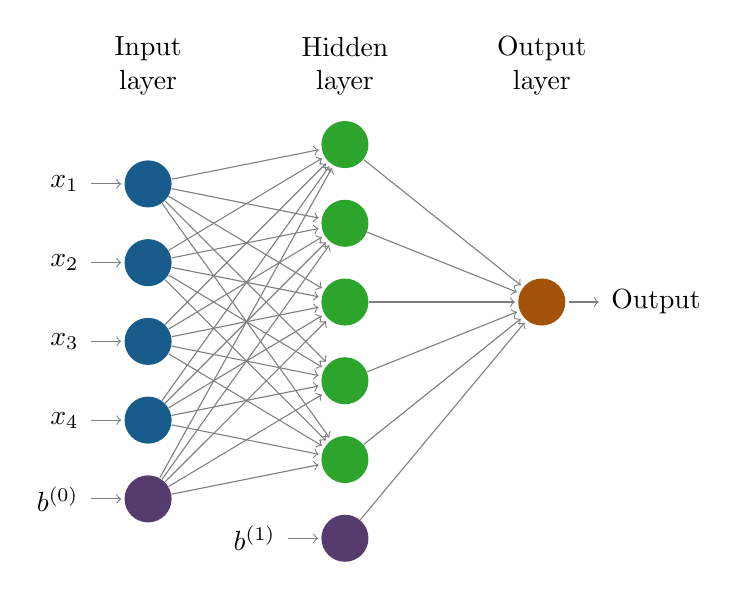
\begin{tikzpicture}[shorten >=1pt,->,draw=black!50, node distance=\layersep]
  \tikzstyle{every pin edge}=[<-,shorten <=1pt]
  \tikzstyle{neuron}=[circle,fill=black!25,minimum size=17pt,inner sep=0pt]
  \tikzstyle{input neuron}=[neuron, fill={rgb:red,0.12156862745098;green,0.466666666666667;blue,0.705882352941177}];
  \tikzstyle{output neuron}=[neuron, fill={rgb:red,1;green,0.498039215686275;blue,0.0549019607843137}];
  \tikzstyle{hidden neuron}=[neuron, fill={rgb:red,0.172549019607843;green,0.627450980392157;blue,0.172549019607843}];
  \tikzstyle{bias neuron}=[neuron, fill={rgb:red,0.580392156862745;green,0.403921568627451;blue,0.741176470588235}];
  \tikzstyle{annot} = [text width=4em, text centered]

  % Draw the input layer nodes
  \foreach \name / \y in {1,...,4}
  % This is the same as writing \foreach \name / \y in {1/1,2/2,3/3,4/4}
  \node[input neuron, pin=left:$x_\y$] (I-\name) at (0,-\y) {};

  \node[bias neuron, pin=left:$b^{(0)}$] (I-5) at (0, -5) {};

  % Draw the hidden layer nodes
  \foreach \name / \y in {1,...,5}
  \path[yshift=0.5cm]
  node[hidden neuron] (H-\name) at (\layersep,-\y cm) {};

  \path[yshift=0.5cm] node[bias neuron, pin=left:$b^{(1)}$] (H-6) at (\layersep,-6 cm) {};

  % Draw the output layer node
  \node[output neuron,pin={[pin edge={->}]right:Output}, right of=H-3] (O) {};

  % Connect every node in the input layer with every node in the
  % hidden layer.
  \foreach \source in {1,...,5}
  \foreach \dest in {1,...,5}
  \path (I-\source) edge (H-\dest);

  % Connect every node in the hidden layer with the output layer
  \foreach \source in {1,...,6}
  \path (H-\source) edge (O);

  % Annotate the layers
  \node[annot,above of=H-1, node distance=1cm] (hl) {Hidden layer};
  \node[annot,left of=hl] {Input layer};
  \node[annot,right of=hl] {Output layer};
\end{tikzpicture}